\documentclass{article}
%%CHINESE_PACKAGE_PLACEHOLDER%%

\usepackage{arxiv}

\usepackage[utf8]{inputenc}
\usepackage[T1]{fontenc}

\usepackage{graphicx}
\usepackage{amsmath}
\usepackage{hyperref}
\AtBeginDocument{
  \providecommand\BibTeX{{
    Bib\TeX}}}

\usepackage{listings}
\lstset{
    float=tp,
    floatplacement=tbp,
    frame=lines,
    comment=[l]{//},
    language=java,
    basicstyle=\footnotesize\ttfamily,
    numbers=left,
    numbersep=2pt,
    numberstyle=\tiny,
    keywordstyle=\bfseries,
    captionpos=b,
    tabsize=3,
    sensitive=true,
}

\usepackage{algorithm}
\usepackage{algorithmicx}
\usepackage{algpseudocode}

\newcommand{\tool}{EnsLLM}
\begin{document}

\title{基于相似性的集成选择方法增强大语言模型代码生成能力}

\author{
 Tarek Mahmud \\
  Texas State University\\
  \texttt{tarek\_mahmud@txstate.edu} \\
   \And
 Bin Duan \\
  The University of Queensland \\
  \texttt{b.duan@uq.edu.au} \\
  \And
 Corina Pasareanu \\
  Carnegie Mellon University \\
  \texttt{pcorina@andrew.cmu.edu} \\
  \And
 Guowei Yang \\
  The University of Queensland \\
  \texttt{guowei.yang@uq.edu.au} \\
}

\maketitle
\begin{abstract}
集成学习在机器学习领域已被广泛用于提升模型的鲁棒性、准确性和泛化能力,但尚未应用于基于大语言模型(LLMs)的代码生成任务。我们提出了一种面向LLMs代码生成的集成方法。该方法不依赖单一模型的输出,而是从不同LLM生成多个候选程序,并通过结构化投票机制选择最可靠的解决方案。投票过程中,我们使用CodeBLEU计算语法和语义相似度,并借助CrossHair的差异行为分析评估行为等价性。通过聚合这些相似度评分,我们选择与候选方案共识最契合的程序。实验表明,在知名HumanEval数据集和更具挑战性的LiveCodeBench数据集上,我们的集成方法始终优于单一LLM,分别达到90.2\%和50.2\%的准确率。相比之下,性能最佳的单一LLM(GPT-4o)准确率分别为83.5\%和43.4\%。此外,即使仅使用免费开源模型,我们的方法仍能分别实现80.5\%和41.6\%的准确率,证明了该方法在资源受限环境下的可行性。
\end{abstract}

\keywords{大语言模型, 代码生成, 集成学习}
\section{引言}
大型语言模型(LLMs)\cite{brown2020language}显著推动了自动化代码生成的发展,使得模型能够根据自然语言提示生成功能正确的程序。近期模型如GPT-4 \cite{gpt4}、CodeLlama \cite{codellama}和DeepSeekCoder \cite{deepseekcoder}在基准数据集上展现出强劲性能,使其在软件开发工作流程中日益普及。这些模型通过对多样化代码库的大规模训练,能够为不同编程语言的各种编程问题生成代码。其生成、补全和重构代码的能力,促成了在软件工程、竞技编程和AI辅助开发环境中的广泛应用。

然而,尽管取得了这些进展,LLMs并非完美无缺,可能产生错误或次优代码,导致语法错误、逻辑缺陷或边缘情况处理缺失\cite{chen2021evaluating}。LLM生成代码的可靠性高度依赖于问题复杂性、训练数据质量以及模型在训练分布之外的泛化能力。即使是最先进的模型如GPT-4,在HumanEval等标准编码基准测试中也仅达到约82\%的功能正确率,而CodeLlama等开源模型的准确率更低(42-50\%)\cite{bubeck2023sparks, ziemniak2023codellama}。这些差异凸显了专有模型与开源模型之间的性能差距,使得确保不同LLMs间的一致性表现具有挑战性。

LLM代码生成的关键挑战在于故障模式的不可预测性。研究发现,LLMs倾向于生成语法合理但功能错误的解决方案\cite{li2022competition}。此外,LLMs难以处理代码中的长程依赖关系,在推理复杂数据结构或多步算法时会出现问题。OpenAI Codex和GitHub Copilot的评估还表明,LLMs可能引入安全漏洞,例如使用已弃用的API、生成不安全的加密实现或未能正确处理边缘情况\cite{pearce2022asleep}。这些局限性使得生成后验证变得至关重要,强化了对系统化评估和筛选正确解决方案方法的需求,然后才能在实际应用中部署。

集成学习在机器学习中已被广泛用于提升模型鲁棒性、准确性和泛化能力\cite{mienye2022survey}。传统集成技术如装袋法、提升法和堆叠法在图像分类、自然语言处理和异常检测等领域取得了成功,但在LLM代码生成中尚未得到充分探索。先前研究表明,即使使用单一模型生成多个解决方案并选择最佳候选,也能显著提升性能——OpenAI的Codex研究中pass@100准确率远高于pass@1便印证了这一点\cite{chen2021evaluating}。受这些研究启发,我们提出\tool,一种基于集成的方法,通过结构化投票机制组合多个LLMs的输出并选择最可靠的解决方案。与依赖单一模型输出不同,\tool\利用多个候选程序,并应用基于相似性的新颖排序方法来评估语法、语义和行为正确性。

具体而言,\tool\整合了CodeBLEU \cite{codebleu}(一种评估LLM生成程序的流行指标)和差分分析来评估生成程序的可靠性。CodeBLEU用于测量候选程序对之间的语法和语义相似性,使得语法语义相似且逻辑一致的解决方案获得更高排名。由于CodeBLEU仅使用程序的静态信息,我们还研究了互补的{\em 基于执行}的差分分析来检测候选对之间的行为不一致性,并在两个候选产生不同输出时生成反例。在本工作中,我们基于属性测试工具CrossHair \cite{crosshair}定义了行为相似性度量用于差分分析(但也可使用其他差分分析方法\cite{hydiff, lahiri2010differential})。结合这两个指标,\tool\计算所有候选的成对分数,聚合每个候选的分数,并选择得分最高的候选作为集成输出程序。

我们在两个成熟的代码生成基准测试(HumanEval \cite{humaneval}和LiveCodeBench \cite{livecodebench})上评估\tool。结果表明,\tool\始终优于单个LLM,在HumanEval上达到90.2\%的准确率,在LiveCodeBench上达到50.2\%,超越了两个数据集中表现最佳的独立模型。此外,即使仅使用免费开源LLMs,\tool\在HumanEval和LiveCodeBench上仍分别取得80.5\%和41.6\%的成绩,证明了其在资源受限环境中的可行性。

本文的主要贡献如下:
\begin{itemize}
    \item 我们提出一种基于集成学习的LLM代码生成方法,通过利用语法、语义和行为相似性来提升可靠性。
    \item 我们设计了一种新颖的投票机制,整合CodeBLEU和CrossHair指标来评估生成程序的语法相似性、语义对齐度和功能正确性。
    \item 在HumanEval和LiveCodeBench基准上进行了大量实验,证明\tool\显著优于单一LLM。通过分析失败案例,我们发现正确程序会相互增强,这支持了我们的假设:独立LLM不太可能犯相同错误。
    \item 实验表明,即使仅使用免费开源LLM,\tool\仍保持有效性,这使其成为无法使用商业模型环境下的可行解决方案。
\end{itemize}
\section{研究背景}


\subsection{集成学习}
集成学习通过组合多个模型来降低方差、偏差和过拟合,从而提升预测准确性。其主要技术包括装袋法、提升法、堆叠法、投票法等。

装袋法 \cite{bagging}(Bootstrap Aggregating)通过在可重复采样的不同数据子集上训练多个模型,并通过平均(回归任务)或多数表决(分类任务)来整合预测结果。随机森林作为决策树集成方法的典型代表,通过这种方式有效降低方差并提升模型稳定性。
提升法 \cite{boosting} 采用顺序训练策略,后续模型不断修正前序模型的预测误差。诸如AdaBoost、GBM和XGBoost等算法通过迭代优化预测结果,重点关注难分类样本以提升准确率。
堆叠法 \cite{stacking} 利用元学习器整合异构基模型的预测结果,通过学习最优组合策略来增强泛化能力。加权平均法根据模型性能分配不同权重,可进一步提升集成系统的稳定性和准确性。

投票法 \cite{kittler1998combining} 通过多数表决(硬投票)或预测概率平均(软投票)来聚合多个模型的输出。当各基模型具有互补性误差时,该方法能产生更具鲁棒性的最终决策。

集成方法能有效克服单一模型的局限性,在分类、回归和生成任务中表现优异。本文提出的\tool\系统,正是基于投票法集成大语言模型来解决代码生成任务。
\subsection{CodeBLEU}
CodeBLEU \cite{codebleu} 是一种专为评估自动生成代码质量而设计的度量标准,它在传统BLEU(双语评估替补)指标的基础上进行了改进,弥补了其在编程语言语境下的不足。标准BLEU广泛应用于自然语言处理领域,通过计算生成文本与参考文本之间n元语法精度的重叠度(即词序列匹配程度),提供了一种简单有效的词汇相似性评估方法。然而,这种方法缺乏对代码结构化特性的深度理解——在编程领域,语法正确性和语义意图的重要性远超过单纯的符号匹配。CodeBLEU通过整合一个多维度评估框架克服了这些局限,该框架能同时捕捉编程的句法、语义和逻辑特征,使其特别适用于代码生成任务的评估。

CodeBLEU的评估包含四个要素。首先,n元语法精度通过比较生成程序与参考程序之间的标记序列(如关键字、标识符)来捕捉词汇相似性。其次,加权n元语法匹配通过赋予关键标记(如函数名相对于标点符号)更高权重来优化词汇准确性。第三,抽象语法树(AST)相似性评估句法结构,通过比较程序构造(如循环或函数调用)的层次化表示来确保句法一致性。第四,数据流相似性分析变量转换与依赖关系,验证不同实现间的逻辑等价性。最终的CodeBLEU分数是这些组分的加权总和,平衡了词汇、句法和语义的保真度。

这种多维度度量标准能够精确排序和筛选程序输出,即使存在表面相似性,也能区分高质量实现与存在缺陷的实现。作为背景知识,CodeBLEU的综合方法为我们提出的方法奠定了基础,我们的方法在其优势之上进行扩展,以增强基于集成的准确且功能可靠解决方案的选择机制。
\subsection{CrossHair}
CrossHair \cite{crosshair} 是一款基于符号执行的Python工具,能够自动发现程序中断言的反例。该工具通过分析函数逻辑、前置条件和不变式,探索不同执行路径以检测传统测试可能遗漏的错误。CrossHair 整合了Python的类型提示和断言语句来动态验证函数行为,使其成为调试和验证正确性的有效工具。

CrossHair 的差异化行为(diffbehavior)功能允许用户通过使用相同输入执行不同版本的函数并进行比较,识别输出结果出现分歧的情况。该功能系统性地探索可能的输入空间,并报告反例——即那些在某个版本中导致意外或错误行为,而在另一版本中表现正常的输入参数。通过突出这些差异,diffbehavior 帮助开发者检测非预期的变更、功能退化或微妙的逻辑错误。该特性在重构或优化复杂函数时尤为实用,能确保修改不会引入新缺陷的同时保持预期行为。
\section{方法}

\begin{figure*}[t!]
    \centering
    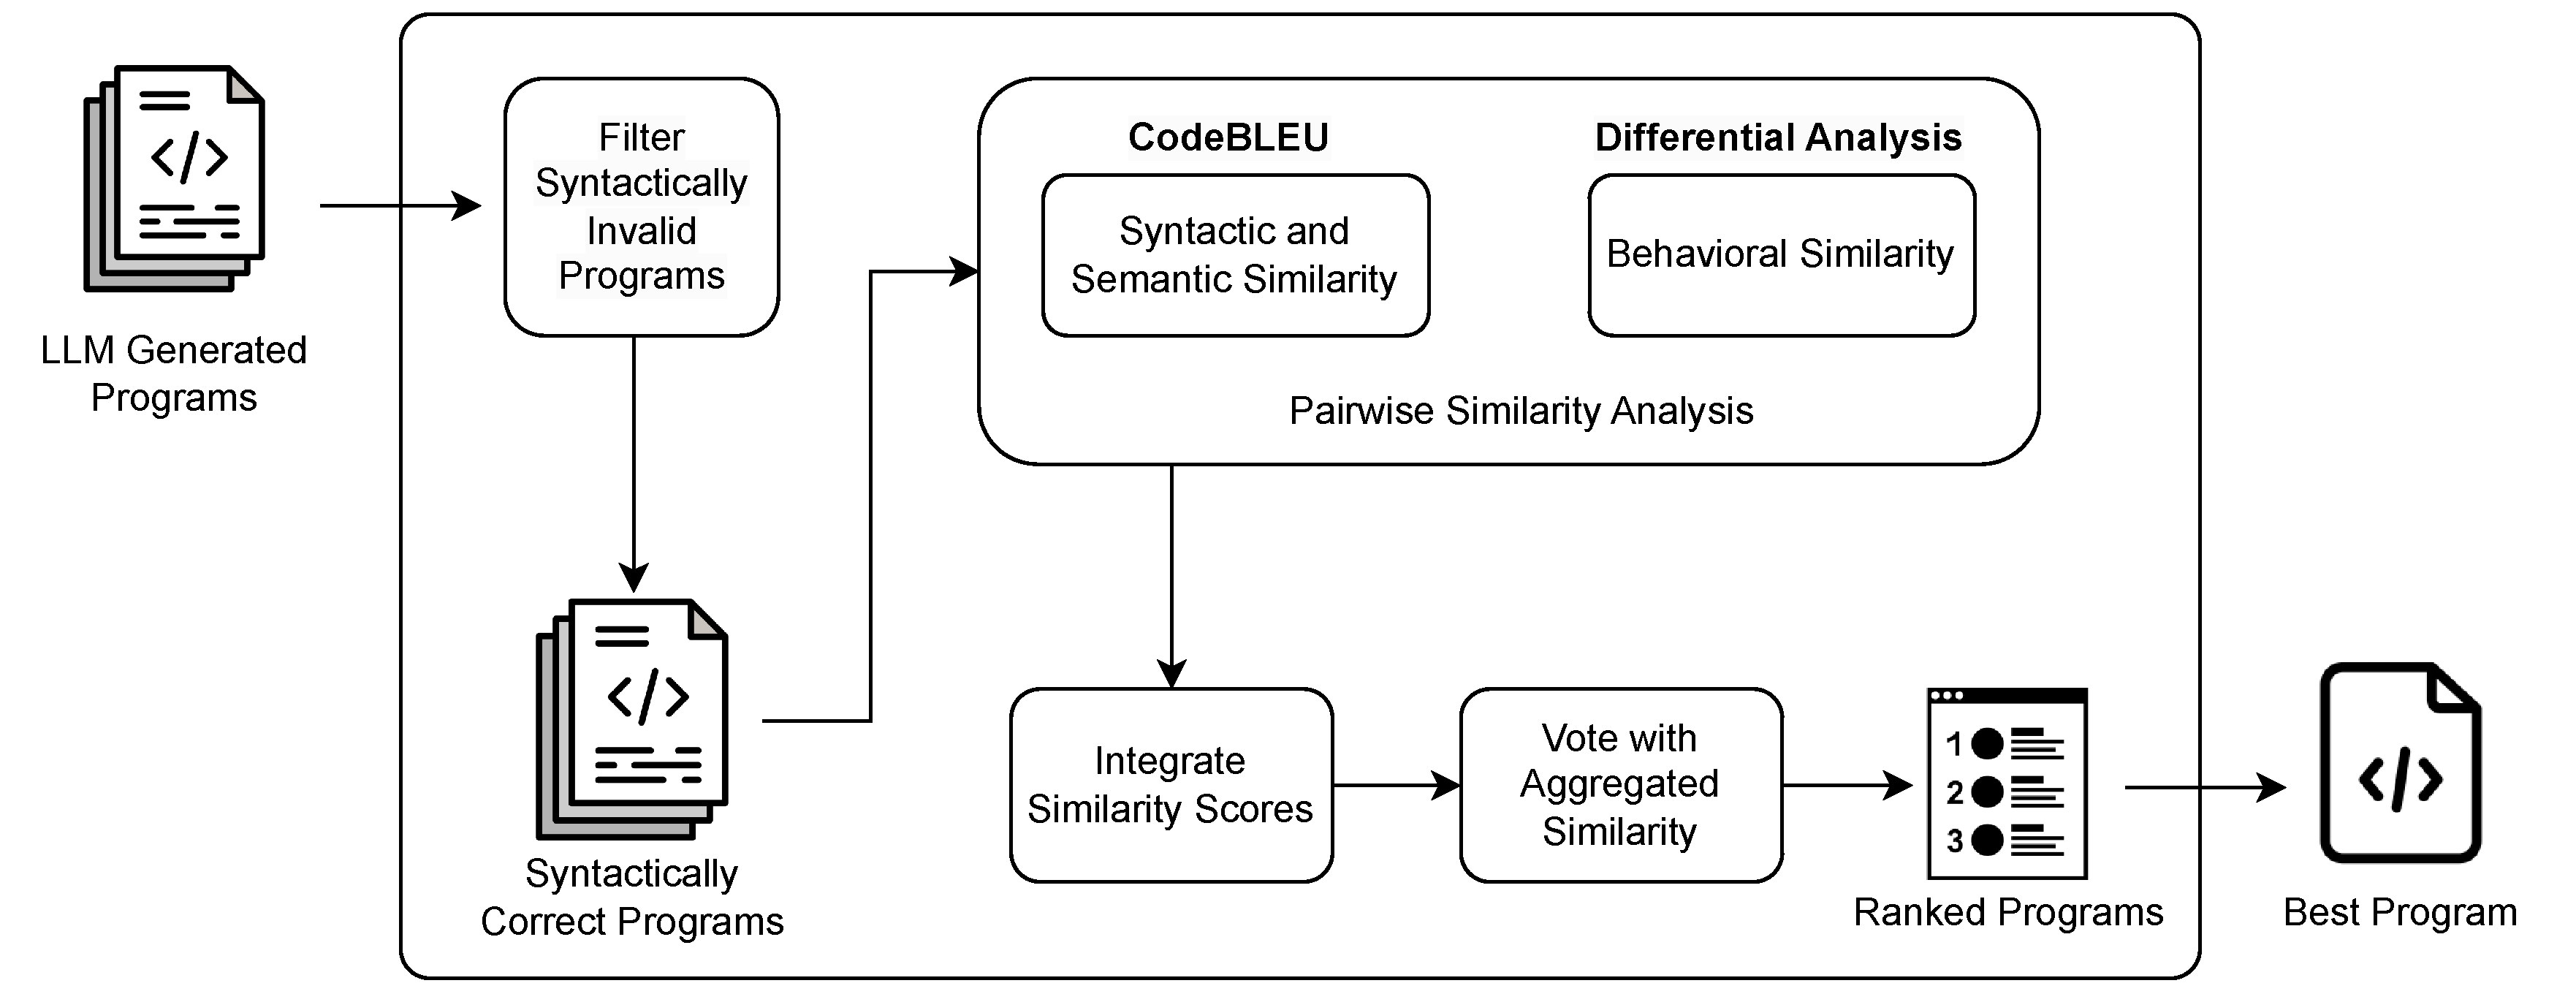
\includegraphics[width=\linewidth]{figure/EnsembledLLM.pdf}
    \caption{\tool 概览}
    \label{fig:overview}
\end{figure*}

我们提出了一种基于大语言模型(LLM)的代码生成集成方法,该方法通过从不同LLM生成多个候选程序,并采用投票机制选择最可靠的解决方案。需要解决的核心挑战是:{\em 如何进行投票?}我们注意到,虽然LLM通常不直接计算置信度值,但这些值可以通过生成过程中分配给每个标记的概率来推断。然而,由于不同LLM的置信度未经过校准,我们不能简单地使用这些值进行投票。针对这一挑战,我们提出了一种基于{\em 语法、语义和行为层面有意义}的程序两两比较的投票机制。

图\ref{fig:overview}展示了我们方法的整体框架。首先过滤掉语法无效的程序,然后通过基于相似性的投票选择最具代表性的解决方案。由于LLM生成的程序常包含幻觉、不完整结构或错位标记,语法过滤是防止相似性计算失真、确保选择过程聚焦于功能可行候选程序的必要步骤。

为评估候选程序间的相似性,我们采用两种互补的度量标准:衡量语法和语义相似性的CodeBLEU指标,以及通过差分分析(CrossHair)测量的行为相似性。CodeBLEU捕捉程序间的词汇、结构和数据流关系,而差分分析则通过生成反例(两个程序输出不一致的情况)来检测功能差异。通过综合这些相似性评分,我们的结构化投票机制能够选出最具代表性的程序作为集成系统的最终输出。
\subsection{语法与语义相似性}
在语法与语义相似性评估方面,我们采用CodeBLEU指标。如前所述,CodeBLEU在传统BLEU基础上扩展了程序特异性特征,能够超越简单的词元重叠,对生成程序的质量和相似性进行更全面的评估。

与仅关注自然语言n元语法匹配的BLEU不同,CodeBLEU针对源代码特性引入了四个评估维度:词汇n元语法匹配(n\_gram\_weight)、句法结构匹配(syntax\_weight)、语义数据流分析(dataflow\_weight)以及词元权重(token\_weight)。在本研究中,我们仅启用syntax\_weight和dataflow\_weight(即赋予非零权重),因为研究重点在于程序的语法结构与语义相似性,而非其文本表象的相似度。通过聚焦这两个维度,我们旨在降低表面词汇相似性的干扰,同时准确捕捉关键的语法模式与语义特征。

\begin{itemize}
    \item \textbf{语法结构匹配(syntax\_weight):}
通过抽象语法树(AST)匹配比较程序的语法组织形式。具有相似语法树的程序在句法上是等价的,即使它们的标记不同。这避免了因格式差异或微小句法变体而对程序进行惩罚。
    \item \textbf{语义数据流匹配(dataflow\_weight):}
分析变量间的数据流依赖关系以评估功能相似性。若两个程序以相同方式操作变量和数据,则视为语义等价,与语法无关。这确保语义相同但词法不同的实现能获得高相似度评分。
\end{itemize}

CodeBLEU在我们的集成方法中发挥着关键作用,通过对生成程序进行两两比对,最终根据聚合相似度分数进行排序。以二分查找任务为例,正确的实现方案——如迭代式(代码清单~\ref{lst:binary_search_iterative})与递归式(代码清单~\ref{lst:binary_search_recursive})——虽然结构相异但功能等价;而错误实现如线性查找(代码清单~\ref{lst:linear_search})则存在效率缺陷或行为偏差(小型语言模型常犯此类错误)。

在进行相似度比对时,CodeBLEU基于抽象语法树的句法度量赋予迭代与递归二分查找0.6的中等相似分,而其数据流分析组件则给出1.0的满分逻辑等价评分。这些正确实现方案在相互比对中形成协同效应,确保其尽管存在语法差异仍能获得稳定高分。相比之下,错误实现与任一正确版本的比对分数显著偏低——例如线性查找与代码清单\ref{lst:binary_search_iterative}的句法相似度仅0.2,与代码清单\ref{lst:binary_search_recursive}为0.3;数据流相似度分别仅为0.3和0.2。这种低分表现确保正确实现能在语法和语义层面形成互补优势。

\begin{lstlisting}[language=Python, caption={Iterative Binary Search Implementation}, label={lst:binary_search_iterative}]
def binary_search_iterative(arr, target):
    left, right = 0, len(arr) - 1
    while left <= right:
        mid = (left + right) // 2
        if arr[mid] == target:
            return mid
        elif arr[mid] < target:
            left = mid + 1
        else:
            right = mid - 1
    return -1
\end{lstlisting}

\begin{lstlisting}[language=Python, caption={Recursive Binary Search Implementation}, label={lst:binary_search_recursive}]
def binary_search_recursive(arr, target, left, right):
    if left > right:
        return -1
    mid = (left + right) // 2
    if arr[mid] == target:
        return mid
    elif arr[mid] < target:
        return binary_search_recursive(arr,
                            target, mid + 1, right)
    else:
        return binary_search_recursive(arr,
                            target, left, mid - 1)

def binary_search(arr, target):
    return binary_search_recursive(arr,
                            target, 0, len(arr) - 1)
\end{lstlisting}

\begin{lstlisting}[language=Python, caption={Linear Search Implementation (Incorrect, as the task requires a Binary Search algorithm)}, label={lst:linear_search}]
def linear_search(arr, target):
    for i in range(len(arr)):
        if arr[i] == target:
            return i
    return -1
\end{lstlisting}

我们方法的核心假设是:语言模型在生成错误程序时不会犯完全相同的错误。这自然降低了正确方案(如代码清单~\ref{lst:binary_search_iterative}和\ref{lst:binary_search_recursive}的二分查找)与错误方案(如代码清单~\ref{lst:linear_search}的线性查找)之间的相似性,同时也降低不同错误实现之间的相似性,从而防止错误程序获得高排名。此外,相似的正确实现将通过强化其共有的语法和语义优势形成协同效应,进一步提升其在集成系统中的综合评分。
\subsection{行为相似性}
语法和语义的相似性并不能保证两个程序在运行时具有完全一致的行为。为解决这一问题,我们采用基于执行的差分分析。本工作中使用CrossHair这一基于属性的测试工具,它通过生成反例(即导致两个程序产生不同输出的输入)来检测行为不一致性。这使得我们能够评估超出CodeBLEU静态计算信息的功能等价性。

对于每对候选程序,\tool\ 运行CrossHair的diffbehavior分析,系统性地探索边界情况以识别差异。反例数量作为逆向相似性度量指标:

\begin{itemize}
    \item 零反例表明两个程序在行为上完全一致,这意味着在所有测试输入下它们产生相同的输出。
    \item 一个或多个反例表明程序表现出不同的行为,突显了逻辑错误或功能差异。
\end{itemize}

为量化行为相似性,我们引入一个通过差分分析评估程序输出一致性的指标。行为相似性度量定义如下:

\begin{equation}
\label{eq:beh_similarity}
\begin{split}
    \text{BSim}_n(P_i, P_j) &=  \left(1 - \frac{\text{MIN}(n, ({\text{cex}}(P_i, P_j))}{n} \right)
\end{split}
\end{equation}

\noindent 其中\( \text{cex}(P_i, P_j) \)表示检测到两个程序产生不同输出的反例数量。由于反例数量可能无限增长,我们通过将其上限设置为自然数\( n \)来标准化影响,防止极端值对相似性分数造成不成比例的影响。该公式确保随着行为不一致性的增加相似度降低,同时通过从1减去的计算方式使功能差异较少的程序获得更高优先级。

通过整合行为相似性信息,我们旨在确保功能不一致的程序获得较低相似性评分,从而提高最终程序选择的可靠性。

\begin{lstlisting}[language=Python, caption={Incorrect Recursive Binary Search Implementation}, label={lst:binary_search_recursive_wrong}]
def binary_search_recursive_wrong(arr, target, left, right):
    if left >= right:
        return -1
    mid = left + (right - left) // 2
    if arr[mid] == target:
        return mid
    elif arr[mid] < target:
        return binary_search_recursive_wrong(arr,
                                    target, mid, right)
    else:
        return binary_search_recursive_wrong(arr,
                                    target, left, mid)
\end{lstlisting}

我们使用差分分析作为CodeBLEU相似性计算的补充。
由于单独的语法和语义相似性(由CodeBLEU计算)不能保证输入输出行为的一致性,差分测试提供了额外的验证层。当比较两个正确实现时(例如迭代和递归的二分查找函数,见代码清单~\ref{lst:binary_search_iterative}和\ref{lst:binary_search_recursive}),它们对于有序列表的所有有效输入始终产生相同输出,不会出现行为偏差。这验证了其正确性并强化了它们在选择过程中的排名。

相比之下,错误实现与正确版本比较时会表现出行为不一致。例如存在缺陷的递归二分查找(代码清单~\ref{lst:binary_search_recursive_wrong})由于错误更新搜索边界而偏离标准二分查找逻辑,可能导致无限递归或遗漏目标值。当正确的迭代(代码清单~\ref{lst:binary_search_iterative})或递归二分查找(代码清单~\ref{lst:binary_search_recursive})与该错误版本比较时,差分分析会分别针对这两个正确实现检测出两个反例。错误程序在与正确实现对比时持续产生反例,导致其在选择过程中排名较低。但需注意仅靠CrossHair(差分分析)并不足够,例如它无法区分代码清单\ref{lst:binary_search_iterative}和\ref{lst:binary_search_recursive}与代码清单\ref{lst:linear_search}的差异,因为它们具有相同的输入输出行为(但代码清单\ref{lst:linear_search}并非理想解决方案,因其未实现二分查找)。
\subsection{语法、语义与行为相似性的集成}

我们通过整合CodeBLEU和基于CrossHair的差分分析,将语法、语义及行为等价性相结合来定义相似性度量指标。

\begin{equation}
\label{eq:similarity}
\begin{split}
   \text{similarity}(P_i, P_j) &= \lambda \cdot \text{CodeBLEU}(P_i, P_j) + (1 - \lambda) \cdot \text{BSim}_n(P_i, P_j)
\end{split}
\end{equation}

\noindent 此处\( \lambda \)为权重因子,用于平衡语法/语义相似度(由CodeBLEU度量)与行为相似度(由BSim\(_n\)度量)。CodeBLEU提供0到1之间的归一化相似度评分,评估程序间词汇、结构及数据流的对齐程度。BSim\(_n\)则通过验证功能正确性进行补充,确保产生相似输出的程序获得更高排名。

CodeBLEU与CrossHair通过捕捉正确性的不同维度形成互补,从而保证更可靠的筛选过程。虽然代码清单~\ref{lst:binary_search_recursive_wrong}存在错误,但使用CodeBLEU评估时其与正确实现的结构相似性较高。由于遵循递归二分搜索结构,与代码清单~\ref{lst:binary_search_iterative}和~\ref{lst:binary_search_recursive}相比可获得相对较高的语法相似度评分。此外,其数据流相似度评分保持中等水平——尽管递归调用中的变量转换存在缺陷,但仍与正确实现中的转换过程相似。这可能导致成对比较时获得较高的CodeBLEU综合评分,若单独使用可能误导排名结果。

然而,CrossHair的反例分析通过直接验证行为正确性有效缓解了该问题。虽然代码清单~\ref{lst:linear_search}作为完全不同的算法在CodeBLEU中获得较低的语法和数据流相似度评分,但其简洁性有助于CrossHair验证预期输出与实际输出的匹配情况。由于线性搜索总能找到目标值,其与代码清单~\ref{lst:binary_search_iterative}和~\ref{lst:binary_search_recursive}的差分分析不产生任何反例,但与代码清单~\ref{lst:binary_search_recursive_wrong}(因错误的索引更新导致特定情况下失败)的差分分析会产生2个反例。这确保即使在错误实现中,CrossHair也能有效区分功能正确性。

通过融合CodeBLEU的结构语义相似度与CrossHair的行为验证,我们的方法确保正确实现之一的代码清单~\ref{lst:binary_search_recursive}获得最高排名。CodeBLEU与CrossHair的协同作用使我们能够过滤得分虚高但错误的解决方案,同时确保选择最健壮的实现。
\subsection{基于聚合相似度的投票选择}

最终,对于每个候选程序,我们通过计算其与集合中所有其他程序的相似度得分之和,得到一个聚合相似度分数。该分数量化了程序与生成候选群体共识的一致性程度,确保优先选择在语法、语义和行为层面保持一致的候选程序。

\begin{equation}
\text{aggregated\_similarity}(P_i) = \sum_{j \neq i} \text{similarity}(P_i, P_j)
\end{equation}

\begin{algorithm}[t!]
\caption{基于聚合成对相似性的投票方法}
\label{alg:ensemble_selection}
\begin{algorithmic}[1]

\Require List of programs \( P = \{P_1, P_2, ..., P_n\} \)
\Ensure The program \( P^* \) with the highest aggregated similarity

\For{each \( P_i \) in \( P \)}
    \For{each \( P_j \) in \( P \) where \( i \neq j \)}
        \State \( \text{similarity}[i][j] \gets \text{Compute\_Similarity}(P_i, P_j) \)
    \EndFor
\EndFor

\For{each \( P_i \) in \( P \)}
    \State \( \text{agg\_sim}[i] \gets 0 \)
    \For{each \( P_j \) in \( P \) where \( i \neq j \)}
        \State \( \text{agg\_sim}[i] \gets \text{agg\_sim}[i] + \text{similarity}[i][j] \)
    \EndFor
\EndFor

\State \( \text{best\_programs} \gets \{ P_i \mid \text{agg\_sim}[i] = \max(\text{agg\_sim}) \} \)

\State \( P^* \gets tie\_breaking(\text{best\_programs}) \)

\State \Return \( P^* \)

\end{algorithmic}
\end{algorithm}

算法~\ref{alg:ensemble_selection}展示了我们基于结构化投票的选择流程,用于从候选程序集中识别最可靠的程序。该算法首先计算程序间的两两相似度,并将结果存储在相似度矩阵中(第$1-5$行);随后通过累加每个程序与其他所有程序的相似度值来计算其聚合相似度分数(第$6-11$行)。具有最高聚合相似度的程序将被选为最优解。若多个程序获得相同最高分,则应用平局裁决机制:当聚合相似度相同时,优先选择CrossHair反例数量较少的程序;若仍持平,则通过随机选择确保决策的确定性,同时保持程序选择的多样性。

选择具有最高聚合相似度分数的程序,能确保所选解决方案在所有生成候选中具备最高的一致性、可靠性和容错性。通过优先选择与群体共识最吻合的程序,我们有效降低了异常值(因语法错误、逻辑缺陷或行为不一致而显著偏离常见模式的程序)的影响。此外,该方法增强了语法、语义及行为层面的可靠性——被选程序不仅与其他高质量候选共享关键语法和语义特征,还表现出最小的行为差异,从而保证正确执行。同时,包含错误逻辑或非预期变体的程序会自然获得较低相似度分数,降低其被选概率。因此,我们的选择机制能有效过滤不可靠输出,同时强化对功能正确、语法语义规范的程序的选择。
\subsection{局限性}

尽管我们的方法显著提高了代码生成准确性,但仍存在若干局限。首先,如果候选程序集中不包含正确解,我们的方法无法独立生成正确程序,只能从现有候选中进行选择。这使得其效果高度依赖于大语言模型生成输出的质量。此外,若"不同模型不会犯相同错误"的假设不成立,且多个模型产生了相似的错误输出,我们的筛选机制可能无法有效剔除这些错误解。

其次,当经过初始语法正确性过滤后仅剩两个程序时,基于成对相似性的投票机制将无法区分二者,因为它们总会获得相同的聚合分数。这一局限源于我们的方法依赖相对排序而非绝对正确性评估。

第三,当多个程序获得相近的聚合相似度分数时,我们的决胜机制会优先选择CrossHair反例较少的程序,但这并不能始终保证正确性。由于CrossHair仅能基于其生成的测试用例识别行为差异,可能无法捕捉更深层次的功能问题,从而导致最终选择的模糊性。
\section{评估}


\subsection{实验设置}
为了评估\tool,我们在两个成熟的程序生成基准测试(HumanEval和LiveCodeBench)上进行了大量实验。目的是评估我们的集成方法相较于独立大型语言模型(LLMs)在选择功能正确程序方面的有效性。
\subsubsection{研究问题}
我们的评估围绕三个关键研究问题展开。
\begin{itemize}
    \item
{\textbf{RQ1: 与独立大型语言模型相比,\tool\ 的性能表现如何?}}
    \\ 我们采用 pass@1 指标衡量功能正确性,并评估 \tool\ 是否比独立模型提高了整体成功率。
    \item
{\textbf{RQ2: CodeBLEU 与 CrossHair 如何分别影响 \tool\ 的准确率?}}
    \\ 通过消融实验评估 CodeBLEU(语法与语义相似度)和 CrossHair(行为等价测试)在筛选正确输出时的独立贡献。
    \item
{\textbf{RQ3: 仅使用免费大型语言模型能获得多少准确率提升?}}
    \\ 我们分析 \tool\ 能否在仅使用开源模型(如 OpenChat、CodeLlama、DeepSeekCoder)的情况下仍保持较高准确率。
\end{itemize}
\subsubsection{基准测试}
\leavevmode\par
为严格评估\tool,我们采用两个广受认可的基准测试集:HumanEval和LiveCodeBench。这些数据集提供了多样化的编程任务,用于评估大语言模型(LLMs)生成功能正确且语法有效程序的能力。

\begin{itemize}
    \item \textbf{HumanEval} \cite{humaneval} 是一个专门用于评估大语言模型生成代码功能正确性的基准测试。它包含164个Python编程问题,每个问题均以结构化格式呈现,包括自然语言提示、函数签名以及用于验证的隐藏测试用例集。这些问题涵盖数学计算、字符串操作、数据结构和逻辑推理等多个领域。由于HumanEval主要关注正确性而非效率或复杂度,生成程序采用pass@k指标进行评估。该指标通过提供的测试用例判断前k个生成方案中是否至少有一个功能正确。凭借其受控的实验设置和标准化评估框架,HumanEval已成为自动化代码生成领域广泛采用的基准测试。

    \item \textbf{LiveCodeBench} \cite{livecodebench} 是一个综合性基准测试,旨在评估大语言模型在多种编程相关任务中的能力。该数据集包含四个独立类别:代码生成、自我修复、测试输出预测和代码执行。在我们的评估中,我们仅关注代码生成子集,其中包含511个覆盖广泛编码场景的编程问题。这些问题比HumanEval更具多样性,包含现实世界的编码任务、API使用、算法挑战和数据结构操作。此外,LiveCodeBench引入了更复杂的问题表述,要求模型不仅要生成语法正确的代码,还需确保API的正确使用和逻辑一致性。与HumanEval类似,pass@k作为主要评估指标,为功能正确性提供了稳健的衡量方式。该数据集的纳入确保\tool\能在更广泛反映真实软件开发场景的编码挑战中得到测试。
\end{itemize}
\subsubsection{基线模型}
\leavevmode\par
我们将\tool\与14种不同的LLM进行对比,包括专有模型和开源模型:
\begin{itemize}
    \item 专有大语言模型:GPT-4o、GPT-4、GPT-3.5、CoPilot、Gemini
    \item 开源大语言模型:OpenChat、CodeBERT、Llama 3.2、Qwen2、Codestral、Gemma 2、DeepSeekCoder、CodeLlama、DolphinCoder
\end{itemize}

专有模型(GPT-4o、GPT-4、GPT-3.5、CoPilot和Gemini)通过官方API访问,提供最先进的代码生成和推理能力。对于开源模型(OpenChat、CodeBERT、Llama 3.2、Qwen2、Codestral、Gemma 2、DeepSeekCoder、CodeLlama和DolphinCoder),我们使用Ollama工具和ollama-python库进行执行。开源模型具有灵活性、透明度和离线可用性等优势,是商业模型的可行替代方案。这种多样化选择实现了平衡比较,在代码生成场景下同时评估尖端专有模型和免费可用的替代方案。
\subsubsection{实现方法}
\leavevmode\par
\tool 的实现采用结构化集成流程,通过聚合多个大语言模型(LLM)的输出以提升生成程序的可靠性与正确性。该流程首先从14个不同的LLM收集候选解决方案,每个模型针对给定编程问题独立生成响应。这种生成多样性提供了广泛的潜在正确实现方案,提高了选择高质量解决方案的概率。然而在进行选择前,所有生成程序都需通过PyLint进行语法验证,确保过滤掉语法无效的解决方案,从而在流程早期减少错误候选。

为确定功能最正确的程序,\tool 采用基于相似性的选择方法,结合CodeBLEU进行语法语义相似度分析,以及CrossHair进行行为正确性评估。CodeBLEU通过分析抽象语法树(AST)和数据流,评估不同候选方案在词汇、语法和语义层面的对齐程度,确保与高质量实现语法语义相似的解决方案获得更高排名。同时,CrossHair通过基于反例的行为分析进行补充,识别程序在不同输入下函数输出的差异表现。在多样化测试用例中保持一致的解决方案将获得更高评分。最终选择基于整合两种评估机制的聚合相似度分数,确保所选方案同时满足语法语义正确性与功能可靠性要求。本实验中,\tool 的实现参数设为$\lambda = .5$和$n = 10$。

为验证所选方案的正确性,\tool 会针对基准数据集提供的单元测试用例执行该方案。HumanEval和LiveCodeBench中的每个编程问题都关联一组预定义测试用例,用于评估生成程序是否产生预期输出。本评估采用pass@1作为核心指标,即对每个编程问题仅从LLM生成一个程序解决方案。该指标通过执行基准数据集中的预定义单元测试用例,评估单次生成方案功能正确的概率。使用pass@1提供了严格且现实的性能度量,因其反映了模型在首次尝试时生成正确解决方案的能力,而无需依赖多次输出。这种方法高度契合现实编码场景,开发者通常寻求即时可用的解决方案而非针对单一问题生成多个备选方案。

所有实验均在配备NVIDIA GeForce RTX 4060(16GB显存)、32GB内存和英特尔酷睿i7(第12代)处理器的高性能计算系统上运行,操作系统为Windows 11。GPU加速技术的使用确保了多LLM的高效执行,显著减少大规模基准测试任务的计算时间。该实验配置支持可扩展且可重复的测试,确保\tool 的性能在真实条件下得到严格评估。
\subsection{实验结果}

\subsubsection{RQ1: 与独立大语言模型相比,\tool\ 表现如何?}
\begin{table}[t!]
    \centering
    \caption{\tool\ 与独立大语言模型在 HumanEval 和 LiveCodeBench 基准上的性能对比(pass@1 指标)。(F) 表示免费模型,括号内数值为可达到的准确率。}
    \label{tab:elfcg_performance}
    \begin{tabular}{|l|c|c|}
        \hline
        \textbf{LLM} & \textbf{HumanEval (\%)} & \textbf{LiveCodeBench (\%)} \\
        \hline
        GPT-4o         & 83.5  & 43.4  \\
        GPT-4          & 82.3  & 42.2  \\
        GPT-3.5        & 76.8  & 39.1  \\
        CoPilot        & 74.4  & 41.6  \\
        OpenChat (F)      & 71.3  & 37.3  \\
        CodeBert (F)      & 68.9  & 37.2  \\
        Llama 3.2 (F)     & 68.9  & 36.7  \\
        Gemini         & 66.5  & 36.1  \\
        Qwen2 (F)         & 62.1  & 36.4  \\
        Codestral (F)     & 59.2  & 37.2  \\
        Gemma 2  (F)      & 52.1  & 31.3  \\
        DeepSeekCoder (F)  & 50.6  & 25.6  \\
        CodeLlama  (F)     & 42.7  & 23.4  \\
        DolphinCoder (F)   & 34.8  & 22.2  \\
        \hline
        \textbf{\tool\ (All)} & \textbf{90.2 (90.9)} & \textbf{50.2 (53.8)} \\
        \hline
        \textbf{\tool\ (Top 5)} & \textbf{87.2 (90.9)} & \textbf{48.3 (53.8)} \\
        \hline
        \textbf{\tool\ (All Free)} & \textbf{80.5 (83.2)} & \textbf{41.6 (44.1)} \\
        \hline
    \end{tabular}
\end{table}
\leavevmode\par
为评估\tool的有效性,我们使用pass@1指标将其在HumanEval和LiveCodeBench数据集上的表现与独立大语言模型进行对比。目的是验证\tool是否通过集成选择策略提升了单个模型的准确率。表\ref{tab:elfcg_performance}展示了各独立大语言模型及\tool在三种模式下于HumanEval和LiveCodeBench的表现。其中\tool(全部)表示使用本研究所涉全部大语言模型时的结果。

括号内标注的"可达准确率"指集成选择方法在理想选择策略下可能达到的最大准确率,其定义为:在集成模型中至少有一个大语言模型能生成正确解的问题占比。由于\tool不生成新程序而是从多个大语言模型输出中选择最佳候选方案,其性能上限本质上受限于生成候选方案中正确解的存在情况。数学上,若使用包含\( N \)个大语言模型的集成,对于包含\( M \)个问题的基准数据集,其中\( C \)表示至少有一个大语言模型生成正确解的问题数量,则可达准确率计算公式为:
\[
\frac{\text{C}}{M} \times 100
\]
该指标给出了\tool性能的理论上限。本研究中,HumanEval和LiveCodeBench的可达准确率分别为90.9\%和53.8\%,这意味着即使采用完美选择机制,系统也无法超越这些值,因为剩余问题在现有大语言模型生成方案中不存在正确解。

HumanEval上表现最佳的独立模型是GPT-4o(83.5\%),其次是GPT-4(82.3\%)和GPT-3.5(76.8\%)。LiveCodeBench中准确率最高的独立模型同样是GPT-4o(43.4\%),随后是GPT-4(42.2\%)和CoPilot(41.6\%)。

\tool在HumanEval上达到90.2\%的准确率,超越了所有独立模型(包括表现最佳的GPT-4o的83.5\%)。这一结果表明,通过整合多个模型并选择最可靠方案,\tool能突破单一LLM的性能极限。此外,\tool在LiveCodeBench上取得50.2\%的准确率,显著优于最佳独立模型GPT-4o的43.4\%。鉴于LiveCodeBench问题的挑战性,这一提升凸显了集成选择方法在处理复杂编程任务时的有效性。

针对HumanEval基准的失败案例分析显示:在164个案例中有121例至少两个模型生成正确答案,且\tool在这些情况下均成功选择正确程序。这验证了我们的假设——在基于相似性的集成方法中,正确程序会相互补充从而强化选择效果。其余问题中,28例至少有一个模型生成正确程序,\tool正确识别了其中27例。唯一失败案例源于三个大语言模型生成了相似错误程序,这进一步支持了"独立大语言模型不易犯相同错误"的假设。

通过整合多个大语言模型并应用结构化集成策略,\tool相较独立模型实现了显著提升,尤其在LiveCodeBench上比最佳独立模型高出近7个百分点。如表\ref{tab:elfcg_performance}所示,\tool始终优于所有独立大语言模型,证明集成选择方法能显著增强代码生成的功能正确性。这些结果进一步表明:独立大语言模型受限于个体能力,而\tool有效整合了它们的优势,从而在不同问题领域实现更高准确率和更可靠的代码生成。

为深入分析模型选择的影响,我们评估了替代配置\tool(前5),该配置仅选择表现最佳的五个模型子集而非全部可用模型。该设置在HumanEval和LiveCodeBench上分别达到87.2\%和48.3\%的准确率,对应可达准确率为90.9\%和53.8\%。结果表明即使采用有限模型子集,EnsLLM(前5)也能接近可达准确率上限;同时说明未被纳入\tool(前5)但包含在\tool(全部)中的低性能模型确实对集成性能有重要贡献。
\begin{table}[t!]
    \centering
    \caption{消融实验展示CodeBLEU与CrossHair对准确率的贡献。}
    \label{tab:ablation_codebleu_crosshair}
    \begin{tabular}{|l|c|c|}
        \hline
        \textbf{$\lambda$} & \textbf{HumanEval (\%)} & \textbf{LiveCodeBench (\%)} \\
        \hline
        1 & 85.9 & 49.5 \\
        .75 & 87.2 & 49.5 \\
        .5 & \textbf{90.2} & \textbf{50.2} \\
        .25 & 89.6 & 48.4 \\
        0 & 89.6 & 47.9 \\
        \hline
    \end{tabular}
\end{table}
\begin{table*}[t!]
    \centering
    \caption{不同CodeBLEU权重配置对准确率的影响。}
    \label{tab:codebleu_variants}
    \scalebox{0.8}{
    \begin{tabular}{|l|c|c|}
        \hline
        \textbf{配置方案} & \textbf{HumanEval (\%)} & \textbf{LiveCodeBench (\%)} \\
        \hline
语法权重 = 0.25,数据流权重 = 0.25,n元语法权重 = 0.25,词元权重 = 0.25 & 85.4 & 46.1 \\
        语法权重 = 0.5,数据流权重 = 0.25,n元语法权重 = 0.25 & 86.0 & 46.4 \\
        语法权重 = 0.25,数据流权重 = 0.5,n元语法权重 = 0.25 & 86.6 & 46.4 \\
        语法权重 = 0.25,数据流权重 = 0.75 & 89.0 & 49.5 \\
        语法权重 = 0.5,数据流权重 = 0.5 & 89.0 & 49.5 \\
        \hline
    \end{tabular}}
\end{table*}
\subsubsection{RQ2:CodeBLEU与CrossHair如何分别影响\tool的准确率?}

\leavevmode\par
公式\ref{eq:similarity}定义了统一相似度度量方法,该方法通过权重因子\(\lambda\)平衡代码语法/语义相似度与行为等价性,整合了CodeBLEU与行为相似度(BSim\(_n\))。CodeBLEU捕捉词汇、句法和语义层面的对齐,而BSim\(_n\)则通过测量候选程序间的行为差异来评估功能正确性。

为确定CodeBLEU与BSim\(_n\)的最佳平衡点,我们通过调整\(\lambda\)进行消融实验,并在HumanEval和LiveCodeBench数据集上评估准确率(表\ref{tab:ablation_codebleu_crosshair})。结果显示当\(\lambda = 0.5\)时,两个数据集均达到最高准确率(HumanEval 90.2\%,LiveCodeBench 50.2\%),这表明语法/语义相似度与行为相似度的均衡加权能产生最鲁棒的生成程序选择方案。

当\(\lambda = 1\)(完全依赖CodeBLEU)时,HumanEval准确率降至85.9\%,LiveCodeBench降至49.5\%,说明忽略行为正确性会导致功能错误。相反,当\(\lambda = 0\)(完全依赖BSim\(_n\))时,HumanEval准确率为89.6\%,但LiveCodeBench降至47.9\%,表明缺乏语法/语义对齐时行为检查的局限性。这些结果证实结构相似性与行为正确性缺一不可,二者均衡加权可获得最佳综合表现。

为深入分析CodeBLEU的影响,我们探索了其四个相似度组件的加权策略:词汇相似度、句法相似度、数据流相似度和词元重要性权重。我们系统测试了所有可能的权重组合对准确率的影响。表\ref{tab:codebleu_variants}仅展示优于基线(所有组件均加权为0.25)的配置。当四个矩阵均采用0.25等权时,HumanEval准确率为85.4\%,LiveCodeBench为46.1\%,说明均衡权重虽能获得合理精度,但并非所有问题类型的最优解。

将权重调整为侧重句法与数据流相似度(syntax\_weight = 0.5,dataflow\_weight = 0.5)后,HumanEval准确率提升至89.0\%,LiveCodeBench提升至49.5\%。这表明优先考虑句法对齐和语义等价能获得更好的选择性能。类似地,采用syntax\_weight = 0.25和dataflow\_weight = 0.75的配置也获得相近结果,进一步证实增强语义正确性权重可提高整体准确率。

这些结果表明:词汇相似度和词元重要性权重对正确性验证贡献较小,而句法和数据流分析是选择高质量代码的关键。降低词汇相似度权重可避免模型选择文本相似但功能错误的解决方案,从而提升\tool的整体鲁棒性。

本研究的结论证实:CrossHair能有效确保行为正确性,而CodeBLEU对排序语义相似且句法规范的程序至关重要。二者联合使用时性能最优,因其形成互补优势。此外,优化CodeBLEU权重分配(优先考虑句法和数据流相似度)可进一步提升准确率。

为确定\( n \)的最优值,我们测试了\( n \)取值5至10时对准确率的影响。结果显示当\( n \)介于6至10时准确率最高,而\( n < 6 \)会导致性能显著下降。具体而言,当\( n < 6 \)时准确率降至89.2\%,说明较低的\( n \)值无法捕捉足够的行为差异,降低选择过程的有效性。

这些发现强化了以下结论:结合语法与行为正确性的方法对实现\tool的最高准确率至关重要。通过微调CodeBLEU权重并整合CrossHair进行功能验证,\tool\能有效提升跨领域代码生成的可靠性。
\subsubsection{RQ3:仅使用免费LLM能获得多少准确率提升?}

\leavevmode\par
为评估\tool\在仅使用免费LLM时的有效性,我们采用开源模型(而非GPT-4o、CoPilot等专有模型)组成的集成进行实验。该研究旨在确定\tool\在不依赖高资源商业模型的情况下,是否仍能保持竞争优势。

表\ref{tab:elfcg_performance}显示,当仅使用免费模型时,性能最佳的独立模型是OpenChat,其在HumanEval和LiveCodeBench上的准确率分别为71.3\%和37.3\%。通过为每个问题选择最优免费模型所能达到的理论上限准确率,在HumanEval上为83.2\%,在LiveCodeBench上为44.1\%。这表明虽然免费模型的个体性能弱于专有模型,但通过优化选择策略仍可获得较高准确率。

\tool\仅使用免费模型时,在HumanEval和LiveCodeBench上分别实现了80.5\%和41.6\%的准确率。这证明即使无法使用高端专有模型,\tool\仍能通过集成多样化开源LLM显著提升准确率。相较于最佳独立免费模型,\tool\在HumanEval上获得近9个百分点的提升,在LiveCodeBench上提升4.3个百分点,凸显了集成方法对提升功能正确性的有效性。

实验结果证实,\tool\仅使用免费模型仍能保持强劲性能,显著优于单一开源LLM。虽然其准确率不及包含专有模型的完整集成方案,但在无法使用商业模型时仍是可行替代方案。集成选择机制通过策略性地筛选功能最正确的解决方案,弥补了免费模型的个体性能缺陷,这证明基于集成的代码生成方法在资源受限场景下仍能提升可靠性,适用于专有模型访问受限的情况。

但受限于免费模型(特别是处理LiveCodeBench复杂编码任务时)的能力,\tool\在此设定下的准确率仍低于完整集成方案。HumanEval上\tool\的实际表现(80.5\%)与理论上限(83.2\%)之间的差距表明,通过优化模型选择与权重策略可进一步缩小该差异。
\subsection{有效性威胁}
内部有效性的主要威胁在于CrossHair的检测效果受生成程序复杂度的影响——若程序涉及外部依赖或非确定性行为,CrossHair可能无法识别功能差异。为降低风险,我们同时整合CodeBLEU与CrossHair,确保正确实现能相互验证而错误实现会被标记。

就外部有效性而言,我们的评估仅基于HumanEval和LiveCodeBench,可能无法完全反映现实世界中复杂的编程挑战。但这两个基准在代码生成研究领域被广泛认可,并已用于多项类似研究来评估大语言模型生成程序的功能正确性。其广泛使用性保障了与现有方法的标准化对比,从而缓解了泛化性威胁。

本研究潜在的效度威胁是语言模型选择偏差,因为我们评估的14个大语言模型可能无法完全代表代码生成模型的整体谱系。尽管我们纳入了专有模型与开源模型的混合组合,但更新或更专业的模型可能表现不同,进而影响研究结论。为此我们选择广泛使用的模型,确保比较结果与现有研究和行业实践一致。后续工作将扩展至更广泛的模型集合以进一步验证泛化性。
\section{相关工作}
大型语言模型(LLMs)在自动化代码生成领域取得了显著进展,使得模型能够根据自然语言提示生成功能正确的代码。早期研究引入了基于GPT架构微调的代码生成模型OpenAI Codex,该模型在解决编程问题方面展现出强大能力\cite{chen2021evaluating}。Codex在HumanEval基准测试中实现了28.8\%的pass@1成功率和70.2\%的pass@100成功率,凸显了生成多个输出并择优选取的优势。这一方法催生了GitHub Copilot等工具的诞生,这些工具将基于LLM的代码生成集成至现代集成开发环境\cite{pearce2022asleep}。

尽管取得这些进展,LLMs在正确性、可靠性和效率方面仍存在重大局限。研究表明,即便是GPT-4这样的最先进模型在HumanEval上也仅能达到约82\%的正确率,而CodeLlama等开源模型表现更差,准确率介于42-50\%之间\cite{bubeck2023sparks, ziemniak2023codellama}。LLMs生成的程序往往语法正确但包含逻辑错误、缺失导入或错误的API调用。另一项挑战是安全性——针对GitHub Copilot的研究发现40\%的AI生成程序存在漏洞,引发了在生产代码库中盲目采用LLM输出的担忧\cite{pearce2022asleep}。

为缓解这些问题,研究者探索了多种策略,包括基于人类反馈的强化学习(RLHF)、利用静态分析工具过滤生成程序,以及通过行为验证技术评估正确性\cite{zhao2022large}。在竞技编程领域,DeepMind的AlphaCode证明LLMs可通过生成数千个解决方案并基于测试执行结果筛选来处理算法复杂问题。AlphaCode在Codeforces竞赛中达到人类水平表现,排名超过54\%的人类参赛者\cite{li2022competition}。这表明虽然LLMs仍需验证和后处理,但结合结构化筛选方法时,其生成正确程序的能力显著提升。
本研究的创新点在于引入基于集成学习的方法,通过CodeBLEU评估语法语义相似度,结合CrossHair进行行为验证,从多个LLM生成输出中选择最可靠程序。

除代码生成外,LLMs在自然语言处理和代码相关任务中展现出卓越性能,包括代码补全\cite{deng2022fuzzing, huang2022prompt, jain2022jigsaw, li2022competition, xu2022systematic}、代码合成\cite{liu2023your}和程序修复\cite{xia2023automated}。作为GitHub Copilot底层模型的Codex\cite{codex}\cite{copilot},在将注释自动转换为功能代码方面表现出色,显著提升开发效率,但仍存在细微问题。其他LLMs如BERT\cite{devlin2018bert, tian2023best}、GPT\cite{gpt4, chatGPT, xia2023keep}及各类领域专用模型\cite{le2023invalidator, paul2023automated}也证明了生成语法正确且上下文相关程序的能力。

LLMs在更广泛的软件工程任务中也得到探索,包括自动化缺陷检测、测试用例生成、代码摘要和安全漏洞分析\cite{rahul2023llm, mueller2023automated}。例如,它们可通过函数签名生成测试用例来辅助编写单元测试,在降低开发工作量的同时提高测试覆盖率\cite{mueller2023automated}。此外,LLMs正被集成至代码重构工具,用于提出优化建议并增强代码可读性\cite{zhao2022large}。除这些应用外,LLMs正在变革软件工程工作流,影响软件开发方式\cite{imai2022github, liu2023fill},提升开发者生产力\cite{dakhel2023github, ziegler2022productivity},并辅助安全分析\cite{pearce2023examining}。然而在确保正确性、可维护性和安全性方面仍存在挑战,需要进一步优化验证才能将LLM生成代码可靠集成至实际软件系统。

专家混合(MoE)框架\cite{jordan1994hierarchical}通过门控网络选择最适合每个输入的专家模型,并采用期望最大化算法进行训练。Fedus等人\cite{fedus2021switch}将MoE扩展至具有稀疏激活的万亿参数Switch Transformers,实现了高效语言处理。

集成学习已广泛用于提升软件工程任务的鲁棒性和准确性。研究表明,通过投票、加权平均或元学习组合多个LLM生成方案可增强正确性\cite{zhang2023ensemble, wang2023code}。部分方法采用多模型集成,不同LLMs专攻代码质量的不同方面,从而获得更高功能正确性\cite{wang2023code}。尽管存在这些进展,使用多模型进行选择与优化时计算效率仍是挑战。此外,\tool\ 是首个将多LLM集成应用于代码生成的方法。
\section{结论}

本文提出了\tool,一种基于结构化集成的方法,旨在提升大语言模型生成代码的可靠性与准确性。通过结合CodeBLEU的成对相似性评分(用于语法与语义对齐)和基于CrossHair的差分分析(用于行为一致性验证),我们的方法能够从多个大语言模型生成的候选程序中系统性地筛选出功能正确且语法规范的最佳实现。在HumanEval和LiveCodeBench基准上的实验表明,\tool\ 始终优于单一的大语言模型,这凸显了结构化集成技术在基于大语言模型的代码生成中的潜力。

未来的工作将扩展\tool\ 的代码质量评估维度,引入安全性、性能与可维护性等指标,从而为构建更可靠、适应性强且稳健的AI辅助编程工作流奠定基础。

\bibliographystyle{plain}
\bibliography{Bibliography}

\end{document}
\endinput
